Social media posts are often useful to detect real-time adverse drug reactions(ADR) compared to other available resources such as clinical reports, health records. They can be a valuable tool for pharmaceutical companies to obtain feedback about medication~\cite{plachouras2016quantifying, huynh2016adverse}. Vast number of tweets mentioning drug names and adverse drug re-actions can easily be collected in real-time. Plachouras et al.~\cite{plachouras2016quantifying} reported that from July 9 to September 4, 2014(shown in figure~\ref{fig:daily-tweets-adr}), on average 179K tweets were mentioning drug names and 721 tweets were containing ADRs. They proposed an ecosystem on clinical reports and social media posts can be useful to pharmaceutical companies - shown in figure~\ref{fig:ecosystem-pharmaceutical}.

\begin{figure}[h]
	\centering
	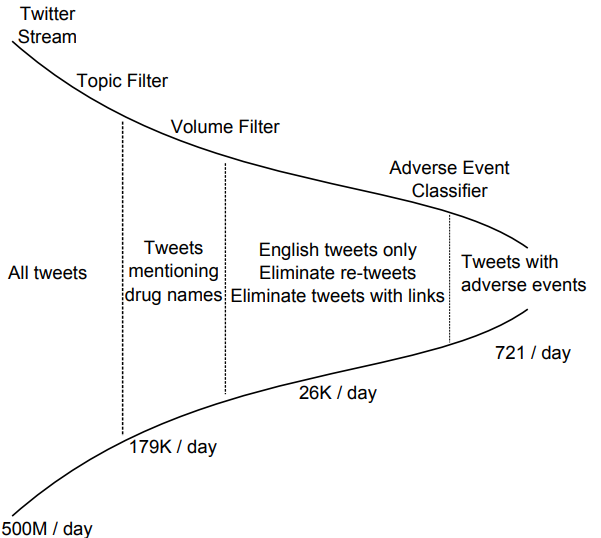
\includegraphics[width=0.99\linewidth]{Figures/g.png}
	\caption{Avg. daily tweets containing ADR from July 9 to September 4, 2014}
	\label{fig:daily-tweets-adr}
\end{figure}

\begin{figure}[h]
	\centering
	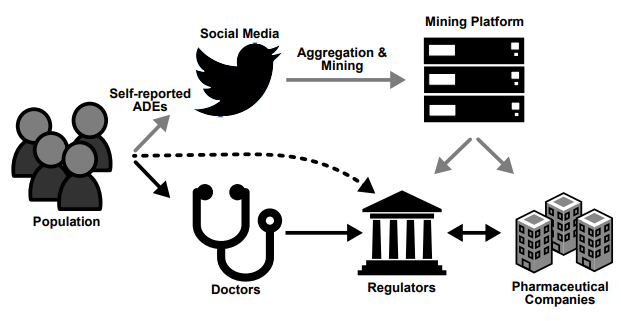
\includegraphics[width=0.99\linewidth]{Figures/j.png}
	\caption{The ecosystem of pharmaceutical companies, regulators, doctors, patients and social media.}
	\label{fig:ecosystem-pharmaceutical}
\end{figure}

The problem of detecting drug names and adverse drug reactions mentioning social media, especially in tweets has been extensively studied in recent years~\cite{weissenbacher2018overview}. Denecke et al.~\cite{DENECKE20091870} performed a content analysis of medical social media data, in particular question \& answer portals, weblogs, reviews, and wikis. The researchers have essentially framed the task of medication name extraction and ADR detection as a binary classification problem. Machine learning techniques are widely used in this task. Deep learning techniques are becoming popular of late. In this review, we will give short reviews of techniques used by various researchers.

Pimpalkhute et al.~\cite{pimpalkhute2014phonetic} noted that preprocessing medication names in social media data often faces the problem of phonetic spelling. Their proposed model found that 50.4 – 56.0 \% of the user comments using only about 18\% of the variants(of spelling). The method, as shown in figure~\ref{fig:model-pimpalkhute}, is based on the intuitive notion that people will tend to spell drug names phonetically. They have used tools and libraries such as the LOGIOS Lexicon Tool\footnote{\url{http://www.speech.cs.cmu.edu/tools/lextool.html}}, Metaphone library\footnote{\url{https://en.wikipedia.org/wiki/Metaphone}} and CMU library\footnote{\url{https://en.wikipedia.org/wiki/CMU Pronouncing Dictionary}}. The considered drug names are available in DrugBank~\footnote{\url{https://go.drugbank.com/stats}}. Limsopatham et al.~\cite{limsopatham2015adapting} used phrase-based machine translation technique~\cite{koehn2003statistical} to translate phrases from ~\textit{Twitter language to formal medical language}.

\begin{figure}[h]
	\centering
	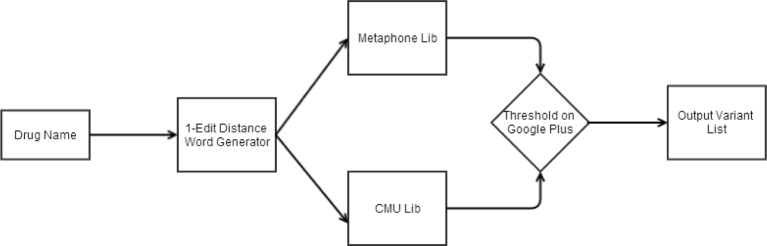
\includegraphics[width=0.99\linewidth]{Figures/m.png}
	\caption{Flow chart of Pimpalkhute et al.~\cite{pimpalkhute2014phonetic} methodology.}
	\label{fig:model-pimpalkhute}
\end{figure}

Sarker et al.~\cite{sarker2016social} proposed a stacking based ensemble classifier to automatically detect whether tweets are abuse or not when they contain specific 4 medication names. The architecture of the methodology is shown in~\ref{fig:model-sarker}. In the ensemble classifier, they used four algorithms - naive bayes(NB), SVM, maximum entropy(ME), and J48, and used various features such as n-gram, abuse-indicating terms, lexicon matches, synonym expansion, word cloud. They concluded that tweets are often ambiguous and impersonal, and a large number of corpus needed for better results. A sample of their annotated data is available\footnote{\url{http://diego.asu.edu/Publications/DrugAbuse_DrugSafety.html}}. In  their  follow-up  work~\cite{sarker2017corpus}, Sarker et al. proposed a corpus  of  267215  Twitter  posts  containing  at least one drug related keyword. They collected this data  over a four-month  period - from  November, 2014  to  February, 2015 and they contain over 250 medication related keywords. This data is available in their website\footnote{\url{http://diego.asu.edu/Publications/Drugchatter.html}}.

\begin{figure}[h]
	\centering
	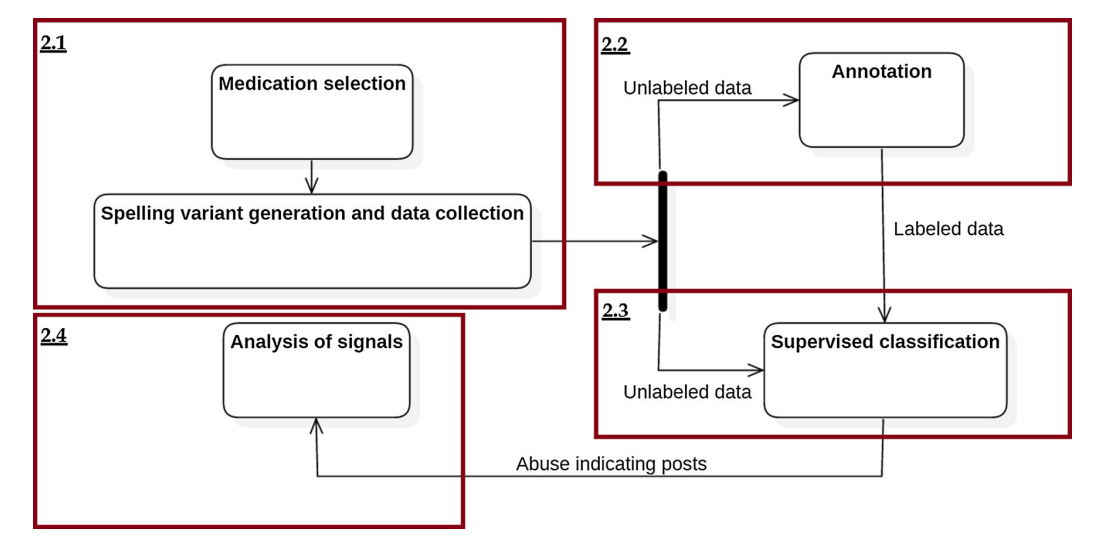
\includegraphics[width=0.99\linewidth]{Figures/h.png}
	\caption{Architecture by Sarker et al.~\cite{sarker2016social}}
	\label{fig:model-sarker}
\end{figure}

Alvaro et al.~\cite{alvaro2015crowdsourcing} explored whether tweets contains information about first-hand medication user experience. They applied crowd sourcing annotation over 1548 tweets whether and annotated them as “First-class experience”, “Tweet written in English language”, and “Tweet about the drug”. The structure of their model is elucidated in figure~\ref{fig:flowchart-alvaro}. There curated corpus is available\footnote{\url{https://github.com/nestoralvaro/JBI Pharmacovigilance/}}.

\begin{figure}[h]
	\centering
	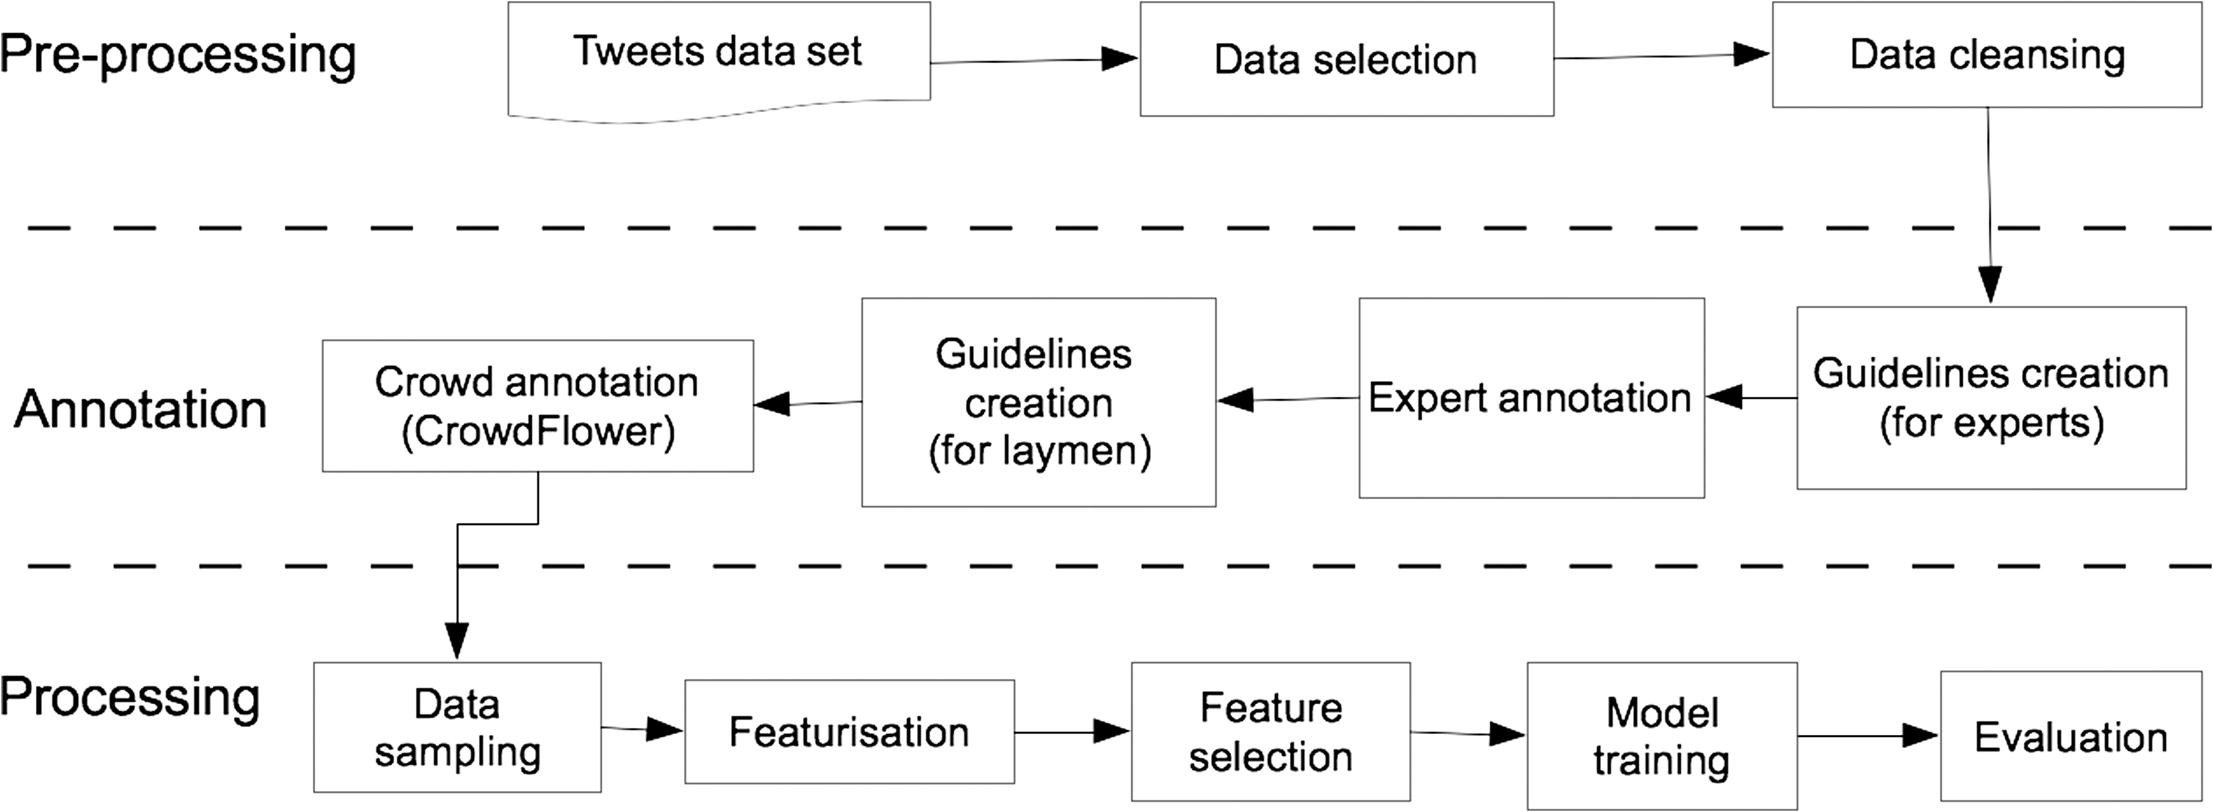
\includegraphics[width=0.99\linewidth]{Figures/n.jpg}
	\caption{Flow chart of Alvaro et al.~\cite{alvaro2015crowdsourcing}’s methodology.}
	\label{fig:flowchart-alvaro}
\end{figure}


Meanwhile, to detect a tweet contains ADR or not, Zhang et al.~\cite{zhang2016ensemble} applied an ensemble algorithm of four classifiers: (1) a concept-matching classifier based on ADR lexicon; (2) a maximum entropy (ME) classifier with word-level n-gram features and TFIDF weighting scheme; (3) a ME classifier based on word-level n-grams using naive Bayes (NB) logcount ratios as feature values; and (4) a ME classifier with word embedding features. They obtain an F-score of 0.4182(positive class). The code of their model is available\footnote{\url{https://github.com/tjflexic/psb-adr}}.


However, these approaches heavily rely on feature engineering and require large amount of expert knowledge. Recently the focus has shifted towards deep learning. Tutubalina et al.~\cite{TUTUBALINA201893} proposed a model based on bidirectional Recurrent Neural Network(RNN) for medical concept normalization in social media. The architecture is illustrated in figure~\ref{fig:architecture-tutubalina}.

\begin{figure}[h]
	\centering
	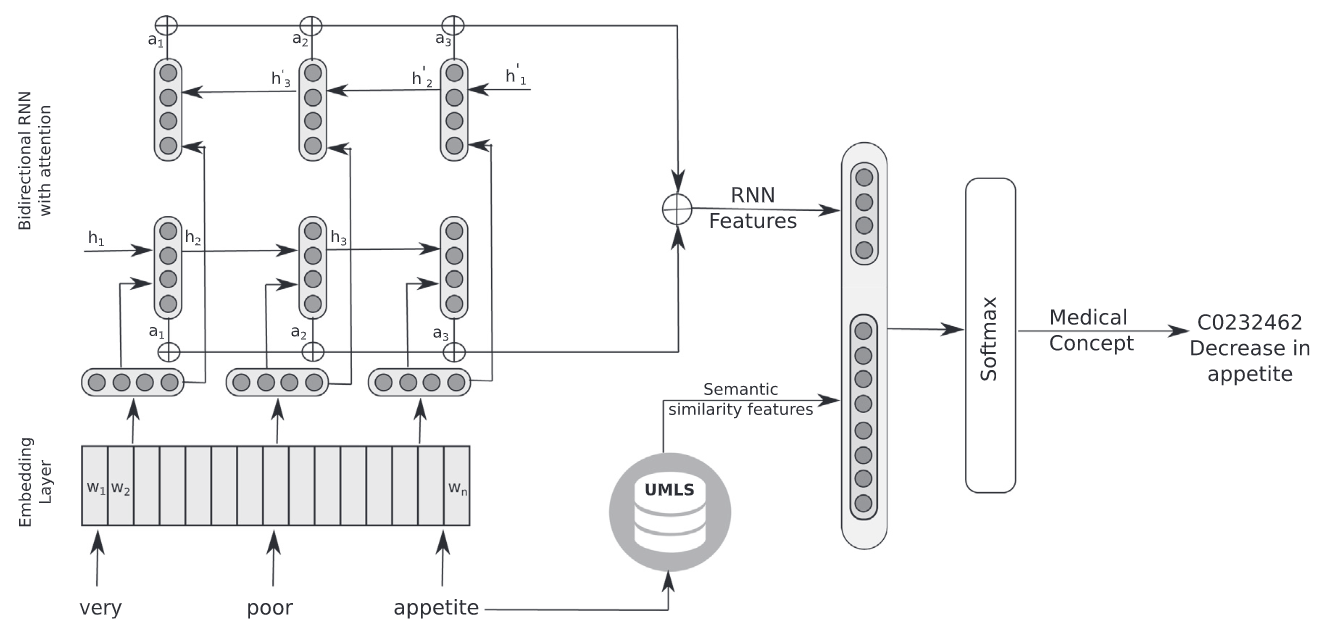
\includegraphics[width=0.99\linewidth]{Figures/f.png}
	\caption{Architecture for medical concept normalization in social media by Tutubalina et al.~\cite{TUTUBALINA201893}.}
	\label{fig:architecture-tutubalina}
\end{figure}

Huynh et al.~\cite{huynh2016adverse} investigated different neural network(NN) architecture for ADR classification. In particular, they applied their data over four algorithms: Convolutional Neural Network (CNN), Recurrent Convolutional Neural Network (RCNN), Convolutional Recurrent Neural Network (CRNN), Convolutional Neural Network with Attention (CNNA). The architecture of these algorithms are shown in the figure 7. They compare model against Zhang et al.~\cite{zhang2016ensemble}’s model and found that CNN obtain highest F-score. The source code the project is available\footnote{\url{https://github.com/trunghlt/AdverseDrugReaction}}.

\begin{figure}[h]
	\centering
	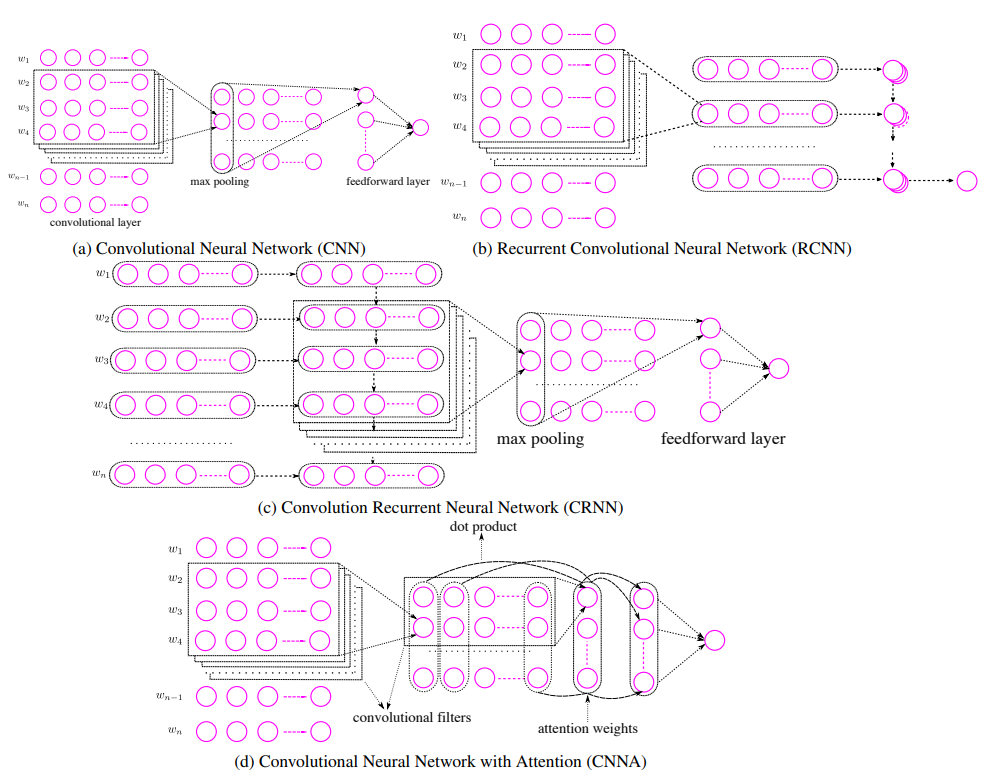
\includegraphics[width=0.99\linewidth]{Figures/e.png}
	\caption{Architecture by Huynh et al.~\cite{huynh2016adverse}.}
	\label{fig:architecture-huynh}
\end{figure}

Lee et al.~\cite{lee2017adverse}, meanwhile, applied a semi-supervised CNN framework for the same task. This model was developed by Johnson et al.~\cite{johnson2015semi}. Lee et al. found that this model outperform a strong state-of-the-art supervised classification model by +9.9\% F1-score. The architecture of the model is shown in the figure~\ref{fig:architecture-lee}. The method works in two phases: (1) unsupervised phrase embedding learning, and (2) integrating the learned embeddings into the supervised training that uses labeled data.

\begin{figure}[h]
	\centering
	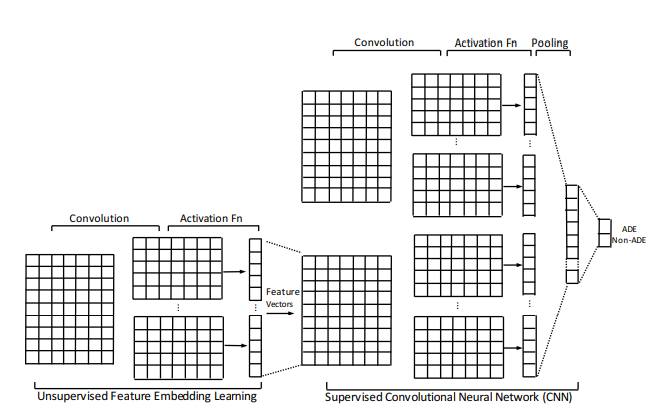
\includegraphics[width=0.99\linewidth]{Figures/l.png}
	\caption{Semi-supervised CNN by Lee et al.~\cite{lee2017adverse}.}
	\label{fig:architecture-lee}
\end{figure}

\begin{figure*}[ht]
	\centering
	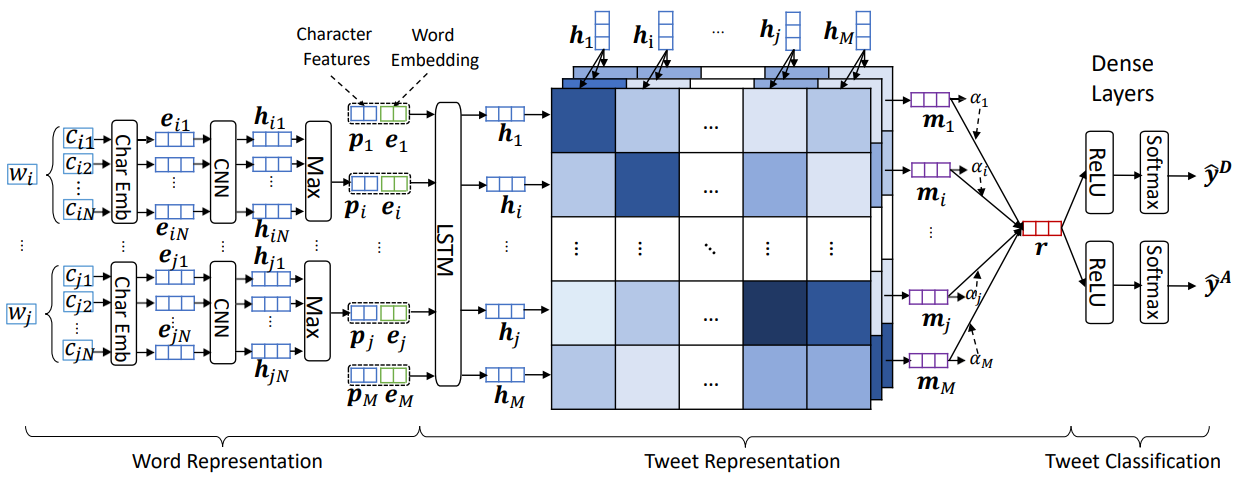
\includegraphics[width=0.99\linewidth]{Figures/k.png}
	\caption{MSA model by Wu et al.~\cite{wu2019msa}.}
	\label{fig:architecture-wu-msa}
\end{figure*}

Wu et al.~\cite{wu2019msa} proposed neural approach using multi-head self-attention (MSA) to jointly detect drug name and adverse drug reaction. Their MSA model has three modules: first, a word representation module, which aims to build the contextual representations of words from the original characters within them; second, a tweet representation module; third, a classification module. The framework of the model is illustrated in the figure~\ref{fig:architecture-wu-msa}.

Weissenbacher et al.~\cite{weissenbacher2019deep} introduced a deep neural networks ensemble method - \textit{Kusuri} - to detect medication names in unbalanced tweets. \textit{Kusuri} is composed of two modules: first, applied 4 different classifiers (lexicon based, spelling variant based, pattern based, and a weakly trained neural network) parallel to discover potential tweets with medication names; second, an ensemble of deep neural networks encoding morphological, semantic, and longrange dependencies of important words in the tweets makes the final decision. The model uses LSTM. The architecture is shown in figure~\ref{fig:architecture-weissenbacher}. This model achieves an F1-score of 0.788 on an extremely unbalanced dataset(98959 tweets, with only 0.26\% mentioning medications). A brief description of 4 algorithms are provided by the authors\footnote{\url{https://tinyurl.com/y47qzbcq}}.

\begin{figure}[h]
	\centering
	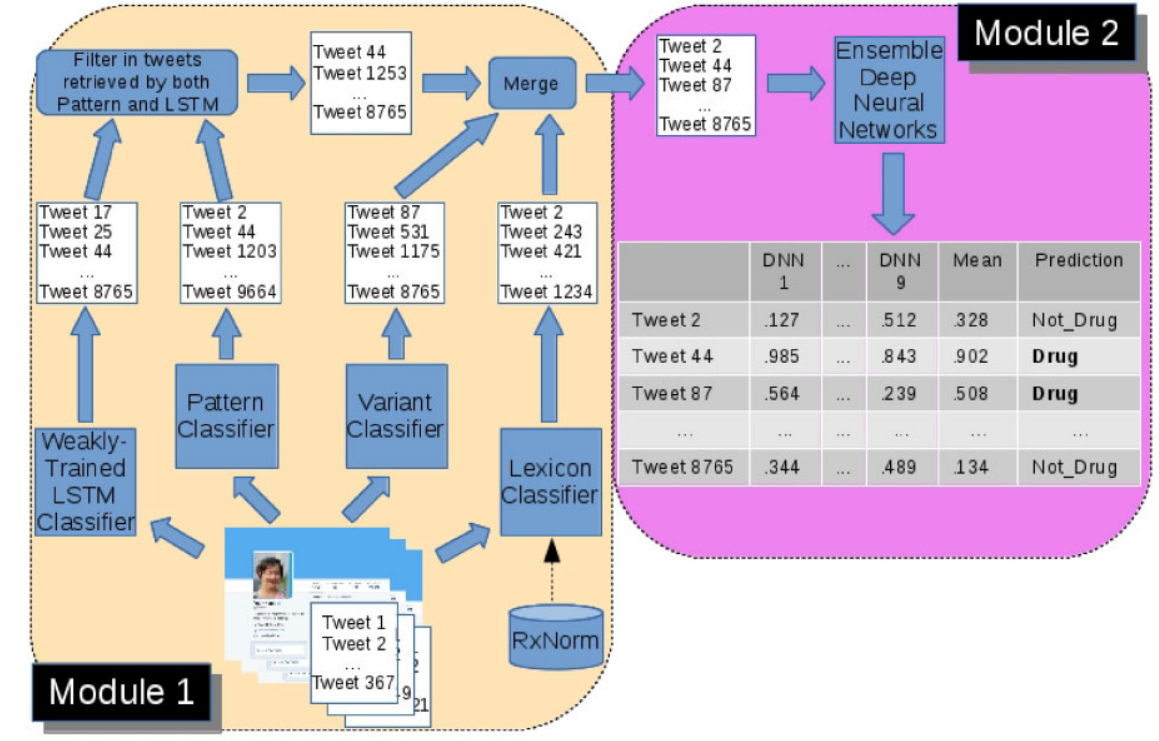
\includegraphics[width=0.99\linewidth]{Figures/a.png}
	\caption{\textit{Kusuri} model by Weissenbacher et al.~\cite{weissenbacher2019deep}.}
	\label{fig:architecture-weissenbacher}
\end{figure}

Researches has been conducted thoroughly to extract medication names from clinical texts and health records~\cite{weeks2020medextractr, kim2020ensemble, ju2020ensemble}.

Ju et al.~\cite{ju2020ensemble} proposed an ensembling system based on neural network to automatically extract adverse drug events and drug related entities from clinical narratives. They firstly pre-processed Electronic Health Records(EHR) using sentence segmentation and tokenization. Then they implemented feature based and neural network-based models to detect ADEs and related medications. The architecture is shown in figure~\ref{fig:architecture-ju}. Their method achieved 92.78\% lenient micro F1-score, with 95.99\% lenient precision, and 89.79\% lenient recall.

\begin{figure}[h]
	\centering
	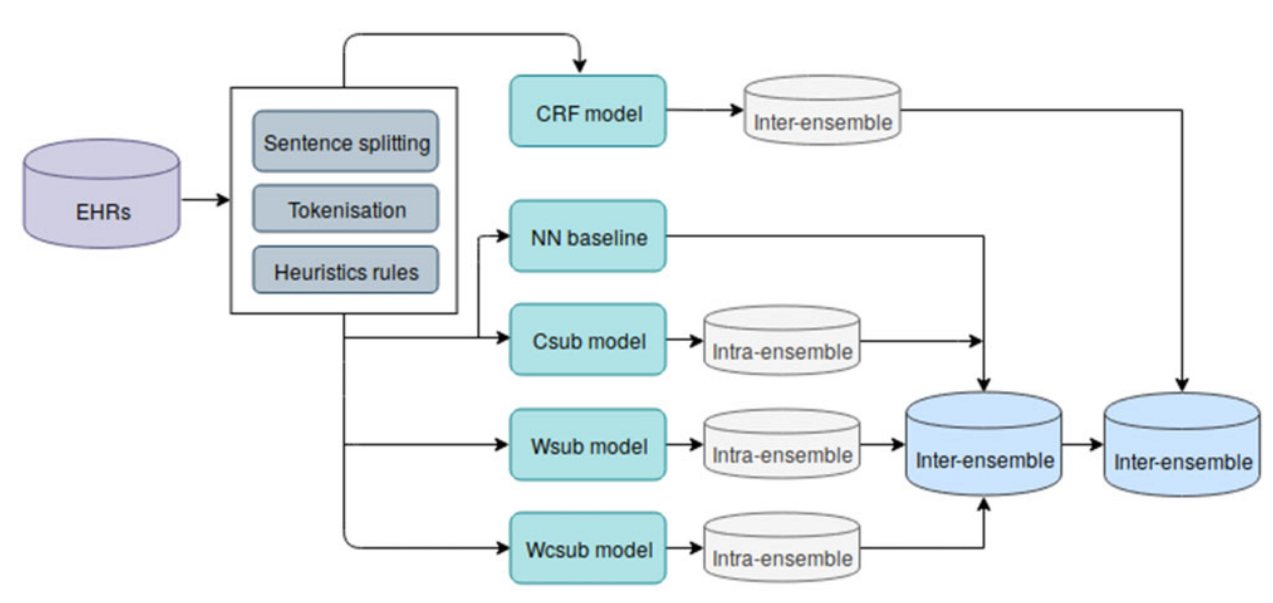
\includegraphics[width=0.99\linewidth]{Figures/c.png}
	\caption{Framework of model by Ju et al.~\cite{ju2020ensemble}.}
	\label{fig:architecture-ju}
\end{figure}

2018 n2c2 shared task on adverse drug events and medication extraction, Kim et al.~\cite{kim2020ensemble} demonstrated that a stacked ensemble with a search-based structured prediction algorithm achieved good performance(an F1 score of 0.9266 on official dataset) by effectively integrating the output of individual classifiers. Their architecture is shown in figure~\ref{fig:architecture-kim}.

\begin{figure}[h]
	\centering
	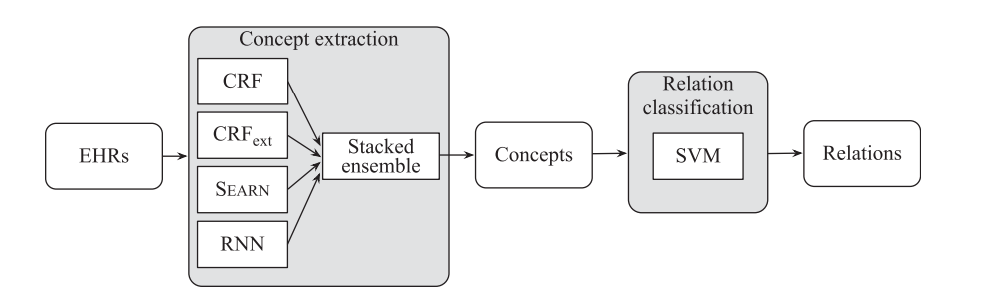
\includegraphics[width=0.99\linewidth]{Figures/i.png}
	\caption{Framework of model by Kim et al.~\cite{kim2020ensemble}.}
	\label{fig:architecture-kim}
\end{figure}

The research of extracting medication names in other languages has been an area of interest as well. Armengol-Estape et al.~\cite{armengol2019pharmaconer} proposed a deep learning-based tool for automatically finding chemicals and drugs in Spanish medical texts.


Alvaro et al.~\cite{alvaro2017twimed} presented a corpus of pharmacovigilance which compromised of 1000 tweets and 1000 PubMed sentences. For the task, they collected 165489 tweets and 29435 PubMed sentences. Their TwiMed pipeline annotation is shown in the figure~\ref{fig:architecture-twimed-alvaro}.

\begin{figure}[h]
	\centering
	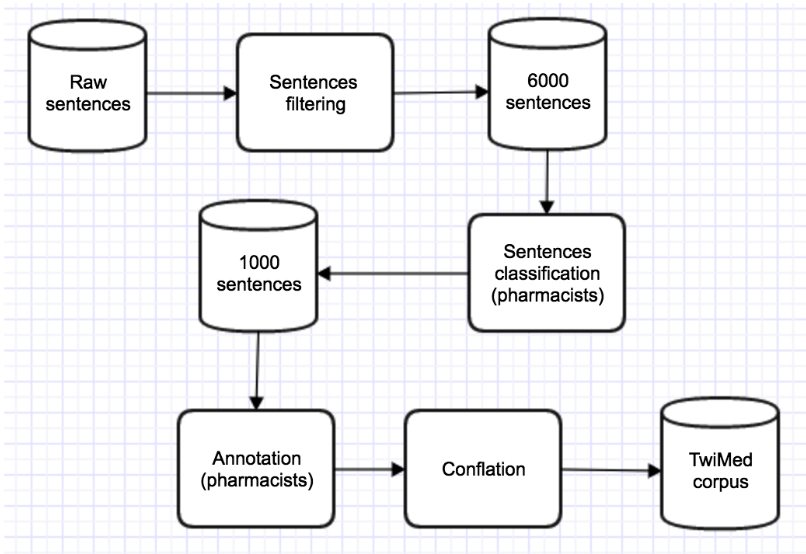
\includegraphics[width=0.99\linewidth]{Figures/b.png}
	\caption{TwiMed annotation pipeline by Alvaro et al.~\cite{alvaro2017twimed}.}
	\label{fig:architecture-twimed-alvaro}
\end{figure}

Klein et al.~\cite{klein2017detecting} focused their study not only on detecting medications but also on distinguishing tweets whether they indicate the user possibly took it or merely mention medication. For this research, they annotated 10260 tweets. The annotation guidelines and a sample of the annotated data are available\footnote{\url{https://healthlanguageprocessing.org/twitter-med-intake/}}. Later, Klein et al.~\cite{klein2019analysis} proposed a corpus of 27941 tweets for medication intake classification. They annotated them in three categories - “intake”, “possible intake”, and “no intake”. O’Connor et al.~\cite{o2020promoting} proposed an annotation guideline when they annotated 16443 tweets mentioning at least 20 abuse-prone medications. The guideline process is shown shown in figure~\ref{fig:annotation-oconnor}. They categorized tweets into four categories: “potential abuse or misuse”, “non-abuse consumption”, “drug mention only”, and “unrelated”. The annotation guideline is available\footnote{\url{https://tinyurl.com/y2zetam9}}.

\begin{figure}[h]
	\centering
	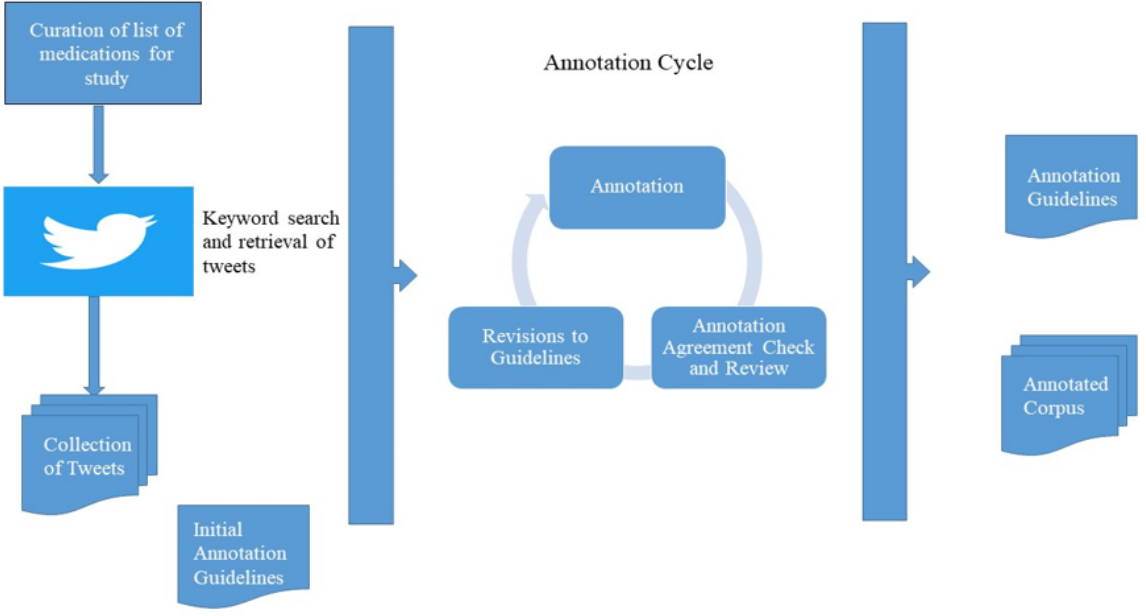
\includegraphics[width=0.99\linewidth]{Figures/d.png}
	\caption{Overview of the creation of the annotation guideline by O’Connor et al.~\cite{o2020promoting}.}
	\label{fig:annotation-oconnor}
\end{figure}
